\documentclass[../thesis/thesis.tex]{subfiles}
\begin{document}
 \chapter{Results}



 \section{Classifier Experiment Set 1}

% TODO: Outline J48 decision tree

\begin{table}
\centering
\begin{tabular}{|l|r|r|r|r|r|r|}
\hline
\textbf{Classifier} & \multicolumn{2}{c|}{\textbf{RMSE}}                                            & \multicolumn{2}{c|}{\textbf{\%}}                                              & \multicolumn{2}{c|}{\textbf{$R^2$}}                                           \\ \hline
                    & \multicolumn{1}{l|}{\textbf{Excl. 0}} & \multicolumn{1}{l|}{\textbf{Incl. 0}} & \multicolumn{1}{l|}{\textbf{Excl. 0}} & \multicolumn{1}{l|}{\textbf{Incl. 0}} & \multicolumn{1}{l|}{\textbf{Excl. 0}} & \multicolumn{1}{l|}{\textbf{Incl. 0}} \\ \hline
\multicolumn{7}{|c|}{Thermosense Replication} \\ \hline                                                                                                                                                                                                                       
KNN (Nominal)       & -                                     & 0.364        & -           & 65.65         & -           & -                                     \\ \hline
KNN (Numeric)       & -                                     & 1.1235       & -           & -             & -           & 0.3766                                \\ \hline
MLP                 & 0.592                                 & -            & -           & -             & 0.687       & -                                     \\ \hline
Lin Reg             & 0.525                                 & -            & -           & -             & 0.589       & -                                     \\ \hline
\multicolumn{7}{|c|}{Nominal Balanced}                                                                                                                         \\ \hline
C4.5                & 0.289                                 & 0.290        & 84.96       & 77.56         & -           & -                                     \\ \hline
K*                  & 0.296                                 & 0.293        & 84.27       & 78.25         & -           & -                                     \\ \hline
MLP                 & 0.359                                 & 0.320        & 70.86       & 72.13         & -           & -                                     \\ \hline
Bayes               & 0.409                                 & 0.368        & 63.76       & 61.52         & -           & -                                     \\ \hline
SVM                 & 0.410                                 & 0.386        & 65.98       & 56.89         & -           & -                                     \\ \hline
0-R                 & 0.471                                 & 0.433        & 32.48       & 24.61         & -           & -                                     \\ \hline
\multicolumn{7}{|c|}{Numeric}                                                                                                                                  \\ \hline
K*                  & 0.423                                 & 0.550        & -           & -             & 0.760       & 0.828                                 \\ \hline
0-R                 & 0.651                                 & 0.972        & -           & -             & -0.118      & -0.129                                \\ \hline
\multicolumn{7}{|c|}{Nominal Unbalanced}                                                                                                                       \\ \hline
C4.5                & 0.314                                 & 0.288        & 82.39       & 82.91         & -           & -                                     \\ \hline
K*                  & 0.304                                 & 0.285        & 82.56       & 82.61         & -           & -                                     \\ \hline
MLP                 & 0.362                                 & 0.286        & 77.14       & 78.69         & -           & -                                     \\ \hline
Bayes               & 0.405                                 & 0.352        & 63.59       & 66.21         & -           & -                                     \\ \hline
SVM                 & 0.398                                 & 0.380        & 67.18       & 57.47         & -           & -                                     \\ \hline
0-R                 & 0.442                                 & 0.415        & 49.74       & 40.37         & -           & -                                     \\ \hline
\end{tabular}
\caption{Classifier Experiment Set 1 Results}
\label{tab:results:set1}
\end{table}

Experimental results from the first set of experiments were overall excellent, results from them can be seen in \Fref{tab:results:set1}. In the unbalanced results when including zero, an accuracy of 82.9\% was observed, and in the balanced results, 78.2\%.  When excluding zero, the unbalanced results achieved 82.5\% in the unbalanced and up to 84.9\% in the balanced results.

\begin{figure}
\centering
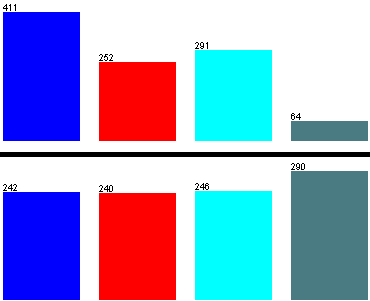
\includegraphics{../diagrams/temp/resample.png}
\caption{Experiment Set 1 Class Distribution Before and After Weka Re-sampling}
\label{fig:results:resample}
\end{figure}

Between the unbalanced and balanced classes when including zero, the ranking of different algorithms remained approximately the same, and consistently dropped in accuracy, with the exceptions being the SVM technique, which increased in accuracy by about 1\% in that instance. The drop in accuracy can be explained mostly by an over-representation of the zero class within the under-balanced data, as well as an underrepresentation of the three class (see \Fref{fig:results:resample}). This is conformed by the fact that in the zero-excluded data, there is much less difference in the balanced and unbalanced set. These biases would enable classes to over-predict and under-predict these two classes respectively and achieve an artificially higher accuracy as a result. As discussed in the Methods, we performed re-sampling inside Weka to compensate for this.

For the numeric representation of the number of people, accuracy was consistently poor. From this data, we can see that all three classifiers used performed consistently poorly, with the Root Mean Square Errors being consistently double or more of comparable nominal results, and with correlation coefficients ($R^2$) indicating poor (or in the case of KNN) very poor correlations.

The two highest accuracy classifiers, C4.5 and K*, achieved quite similar results for both the balanced and unbalanced data while being quite different in implementation. % TODO: Why is this the case

TODO: Discuss and compare this to ZeroR's RMSE. It's RMSE is quite close to some results, is this bad?

\subsection{Individual sub-experiment results}

In addition to the above aggregate classification results, in which each of the nine sub-experiments results are combined and fed into the classifier, each of the sub-experiments has been individually classified with each of the six balanced nominal classifiers above. The results for these classifications can be seen in \Fref{tab:results:set1percent} and \Fref{tab:results:set1rmse}.

TODO: We talk about points of interest in the sub-experiment results and see if we can draw any useful conclusions from them.


\begin{landscape}
\begin{table}
\centering
\begin{tabular}{|l|l|l|l|l|l|l|l|l|l|l|}
\hline
        & \textbf{1}     & \textbf{2}     & \textbf{3}     & \textbf{4}     & \textbf{5}     & \textbf{6}     & \textbf{7}     & \textbf{8}     & \textbf{9}     & \textbf{Avg}   \\ \hline
\multicolumn{11}{|c|}{Nominal}                                                                                                                                                    \\ \hline
KNN     & 0.584          & 0.422          & 0.375          & 0.425          & 0.651          & 0.352          & 0.396          & 0.338          & 0.244          & \textit{0.421} \\ \hline
C4.5    & 0.342          & 0.270          & 0.278          & 0.414          & 0.456          & 0.267          & 0.318          & 0.288          & 0.250          & \textit{0.320} \\ \hline
K*      & 0.305          & 0.249          & 0.260          & 0.412          & 0.407          & 0.245          & 0.299          & 0.265          & 0.196          & \textit{0.293} \\ \hline
MLP     & 0.345          & 0.275          & 0.272          & 0.399          & 0.466          & 0.232          & 0.389          & 0.246          & 0.242          & \textit{0.318} \\ \hline
Bayes   & 0.391          & 0.359          & 0.290          & 0.435          & 0.473          & 0.276          & 0.381          & 0.306          & 0.243          & \textit{0.351} \\ \hline
SVM     & 0.447          & 0.447          & 0.379          & 0.444          & 0.602          & 0.378          & 0.380          & 0.377          & 0.335          & \textit{0.421} \\ \hline
\multicolumn{11}{|c|}{Numeric}                                                                                                                                                    \\ \hline
0-R     & 0.500          & 0.471          & 0.433          & 0.472          & 0.500          & 0.471          & 0.433          & 0.433          & 0.472          & \textit{0.465} \\ \hline
KNN     & 0.726          & 0.707          & 1.044          & 0.934          & 0.593          & 0.531          & 0.899          & 0.585          & 0.829          & \textit{0.761} \\ \hline
K*      & 0.256          & 0.422          & 0.598          & 0.806          & 0.377          & 0.432          & 0.586          & 0.627          & 0.472          & \textit{0.508} \\ \hline
Lin Reg & 0.270          & 0.635          & 0.623          & 0.821          & 0.422          & 0.508          & 0.589          & 0.708          & 0.570          & \textit{0.572} \\ \hline
MLP     & 0.379          & 0.460          & 0.500          & 0.868          & 0.399          & 0.306          & 0.790          & 0.490          & 0.406          & \textit{0.511} \\ \hline
0-R     & 0.409          & 0.762          & 1.009          & 0.986          & 0.507          & 0.829          & 1.014          & 1.043          & 1.012          & \textit{0.841} \\ \hline
Avg     & \textit{0.413} & \textit{0.457} & \textit{0.505} & \textit{0.618} & \textit{0.488} & \textit{0.402} & \textit{0.539} & \textit{0.475} & \textit{0.439} &                \\ \hline
\end{tabular}
\caption{Classifier Experiment Set 1 Individual Sub-experiment RMSEs}
\label{tab:results:set1rmse}
\end{table}
\end{landscape}

\section{Thermosense Comparison}

To aid in comparison with the Thermosense algorithm, in our experiment sets we chose three techniques similar to those used in Thermosense; an Artificial Neural Network (Multilayer Perceptron in Weka), $k$-nearest Neighbors (IBk in Weka) and Linear Regression. Our results for our approximations to their algorithms can be seen in the Thermosense Replication section of \Fref{tab:results:set1}. We also use an experimental setup with 0--3 or 1--3 people, depending on the classifier, just as the Thermosense experiments do. For KNN, it was ambiguous if Thermosense used numeric or a nominal class attributes in their experiments, so we have performed both options above. The specifics of this is discussed in the Methods chapter.

For those experiments where we tried to specifically replicate Thermosense' results, we found consistently poor results that did not come close to meeting the $R^2$ or RMSE values that Thermosense claimed. Their $R^2$ values were in the 0.8 range, while ours range from around 0.3--0.7. This can be put down to a multitude of factors, with one likely explanation being that differences with the \mlx's narrower field of view being difficult for Thermosense' specific algorithmic selections to deal with.

0.141 βS -0.051 β 0.201
F-statistic  3220 R2  0.858
2.44 × 10−187 1.14 × 10−30 9.25 × 10−11

Our Linear Regression (\Fref{eq:linreg}) underperforms particularly when compared to Thermosense' (\Fref{eq:thermolinreg}), as it fails to find an adequate way to weight the two variables, instead opting to basically exclude them from consideration by picking very small weights and adding a large constant factor. We get a correlation of $R^2 = 0.589$ vs Thermosense' $R^2 = 0.858$.

\begin{equation} \label{eq:linreg}
n =  0.0456a + -0.024s + 1.1772
\end{equation}

\begin{equation} \label{eq:thermolinreg}
n =  0.141a + -0.051s + 0.201
\end{equation}

However, for those algorithms we chose ourselves to test, we found results that were comparable or even better than Thermosense. Our nominally classed C4.5 decision tree achieved an balanced RMSE excluding zero of 0.289, compared to Thermosense' best result of 0.346. In the numeric classes, the K* implementation achieved correlations in the same ballpark of 0.760 (excl. 0) and 0.828 (incl. 0), compared to Thermosense' best 0.906 for their ANN.

However, none of the techniques used by Thermosense proved to be the best out of those algorithms tried. The Neural Network and $k$-nearest Neighbors techniques represent the middle-of-the-road of our results, with both being bested by the C4.5 and K* algorithms, which produced RMSEs of 0.289 and 0.298 respectively. Both these results are significantly better than Thermosense's best RMSE of 0.346 for $k$-nearest Neighbors, with our C4.5 algorithm representing a 28\% improvement over that technique.



 \ifcsdef{mainfile}{}{\bibliography{../references/primary}}
\end{document}
